% ****************************************************************************************
% *********************       BASES DE DATOS                  ****************************
% ****************************************************************************************

% =======================================================
% =======         HEADER FOR DOCUMENT        ============
% =======================================================
    % *********   DOCUMENT ITSELF   **************
    \documentclass[12pt, fleqn]{report}                             %Type of docuemtn and size of font and left eq
    \usepackage[margin=1.2in]{geometry}                             %Margins and Geometry pacakge
    \usepackage{ifthen}                                             %Allow simple programming
    \usepackage{hyperref}                                           %Create MetaData for a PDF and LINKS!
    \hypersetup{pageanchor=false}                                   %Solve 'double page 1' warnings in build
    \setlength{\parindent}{0pt}                                     %Eliminate ugly indentation
    \author{Oscar Andrés Rosas}                                     %Who I am

    % *********   LANGUAJE AND UFT-8   *********
    \usepackage[spanish]{babel}                                     %Please use spanish
    \usepackage[utf8]{inputenc}                                     %Please use spanish - UFT
    \usepackage[T1]{fontenc}                                        %Please use spanish
    \usepackage{textcmds}                                           %Allow us to use quoutes
    \usepackage{changepage}                                         %Allow us to use identate paragraphs

    % *********   MATH AND HIS STYLE  *********
    \usepackage{ntheorem, amsmath, amssymb, amsfonts}               %All fucking math, I want all!
    \usepackage{mathrsfs, mathtools, empheq}                        %All fucking math, I want all!
    \usepackage{centernot}                                          %Allow me to negate a symbol
    \decimalpoint                                                   %Use decimal point

    % *********   GRAPHICS AND IMAGES *********
    \usepackage{graphicx}                                           %Allow to create graphics
    \usepackage{wrapfig}                                            %Allow to create images
    \graphicspath{ {Graphics/} }                                    %Where are the images :D

    % *********   LISTS AND TABLES ***********
    \usepackage{listings}                                           %We will be using code here
    \usepackage[inline]{enumitem}                                   %We will need to enumarate
    \usepackage{tasks}                                              %Horizontal lists
    \usepackage{longtable}                                          %Lets make tables awesome
    \usepackage{booktabs}                                           %Lets make tables awesome
    \usepackage{tabularx}                                           %Lets make tables awesome
    \usepackage{multirow}                                           %Lets make tables awesome
    \usepackage{multicol}                                           %Create multicolumns


    % *********   HEADERS AND FOOTERS ********
    \usepackage{fancyhdr}                                           %Lets make awesome headers/footers
    \pagestyle{fancy}                                               %Lets make awesome headers/footers
    \setlength{\headheight}{16pt}                                   %Top line
    \setlength{\parskip}{0.5em}                                     %Top line
    \renewcommand{\footrulewidth}{0.5pt}                            %Bottom line

    \lhead{                                                         %Left Header
        \hyperlink{chapter.\arabic{chapter}}                        %Make a link to the current chapter
        {\normalsize{\textsc{\nouppercase{\leftmark}}}}             %And fot it put the name
    }

    \rhead{                                                         %Right Header
        \hyperlink{section.\arabic{chapter}.\arabic{section}}       %Make a link to the current chapter
            {\footnotesize{\textsc{\nouppercase{\rightmark}}}}      %And fot it put the name
    }

    \rfoot{\textsc{\small{\hyperref[sec:Index]{Ve al Índice}}}}     %This will always be a footer  

    \fancyfoot[L]{                                                  %Algoritm for a changing footer
        \ifthenelse{\isodd{\value{page}}}                           %IF ODD PAGE:
            {\href{https://compilandoconocimiento.com/yo/}          %DO THIS:
                {\footnotesize                                      %Send the page
                    {\textsc{Oscar Andrés Rosas}}}}                 %Send the page
            {\href{https://compilandoconocimiento.com}              %ELSE DO THIS: 
                {\footnotesize                                      %Send the author
                    {\textsc{Compilando Conocimiento}}}}            %Send the author
    }
    
    
    
% ========================================
% ===========   COMMANDS    ==============
% ========================================

    % =====  GENERAL TEXT  ==========
    \newcommand \Quote {\qq}                                        %Use: \Quote to use quotes
    \newcommand \Over {\overline}                                   %Use: \Bar to use just for short
    \newcommand \ForceNewLine {$\Space$\\}                          %Use it in theorems for example
    
    \newenvironment{Indentation}[1][0.75em]                         %Use: \begin{Inde...}[Num]...\end{Inde...}
    {\begin{adjustwidth}{#1}{}}                                     %If you dont put nothing i will use 0.75 em
    {\end{adjustwidth}}                                             %This indentate a paragraph
    \newenvironment{SmallIndentation}[1][0.75em]                    %Use: The same that we upper one, just 
    {\begin{adjustwidth}{#1}{}\begin{footnotesize}}                 %footnotesize size of letter by default
    {\end{footnotesize}\end{adjustwidth}}                           %that's it


    % =====  GENERAL MATH  ==========
    \DeclareMathOperator \Space {\quad}                             %Use: \Space for a cool mega space
    \DeclareMathOperator \MiniSpace {\;}                            %Use: \Space for a cool mini space
    \newcommand \Such {\MiniSpace|\MiniSpace}                       %Use: \Such like in sets
    \newcommand \Also {\MiniSpace \text{y} \MiniSpace}              %Use: \Also so it's look cool
    \newcommand \Remember[1]{\Space\text{\scriptsize{#1}}}          %Use: \Remember so it's look cool

    \newtheorem{Theorem}{Teorema}[section]                          %Use: \begin{Theorem}[Name]\label{Nombre}...
    \newtheorem{Corollary}{Colorario}[Theorem]                      %Use: \begin{Corollary}[Name]\label{Nombre}...
    \newtheorem{Lemma}[Theorem]{Lemma}                              %Use: \begin{Lemma}[Name]\label{Nombre}...
    \newtheorem{Definition}{Definición}[section]                    %Use: \begin{Definition}[Name]\label{Nombre}...

    \newcommand{\Set}[1]{\left\{ \MiniSpace #1 \MiniSpace \right\}} %Use: \Set {Info}
    \newcommand{\Brackets}[1]{\left[ #1 \right]}                    %Use: \Brackets {Info} 
    \newcommand{\Wrap}[1]{\left( #1 \right)}                        %Use: \Wrap {Info} 
    \newcommand{\pfrac}[2]{\Wrap{\dfrac{#1}{#2}}}                   %Use: Put fractions in parentesis

    \newenvironment{MultiLineEquation}[1]                           %Use: To create MultiLine equations
        {\begin{equation}\begin{alignedat}{#1}}                     %Use: \begin{Multi..}{Num. de Columnas}
        {\end{alignedat}\end{equation}}                             %And.. that's it!
    \newenvironment{MultiLineEquation*}[1]                          %Use: To create MultiLine equations
        {\begin{equation*}\begin{alignedat}{#1}}                    %Use: \begin{Multi..}{Num. de Columnas}
        {\end{alignedat}\end{equation*}}                            %And.. that's it!


    % =====  LOGIC  ==================
    \DeclareMathOperator \doublearrow {\leftrightarrow}             %Use: \doublearrow for a double arrow
    \newcommand \lequal {\MiniSpace \Leftrightarrow \MiniSpace}     %Use: \lequal for a double arrow
    \newcommand \linfire {\MiniSpace \Rightarrow \MiniSpace}        %Use: \lequal for a double arrow
    \newcommand \longto {\longrightarrow}                           %Use: \longto for a long arrow

    % =====  NUMBER THEORY  ==========
    \DeclareMathOperator \Naturals  {\mathbb{N}}                     %Use: \Naturals por Notation
    \DeclareMathOperator \Primes    {\mathbb{P}}                     %Use: \Naturals por Notation
    \DeclareMathOperator \Integers  {\mathbb{Z}}                     %Use: \Integers por Notation
    \DeclareMathOperator \Racionals {\mathbb{Q}}                     %Use: \Racionals por Notation
    \DeclareMathOperator \Reals     {\mathbb{R}}                     %Use: \Reals por Notation
    \DeclareMathOperator \Complexs  {\mathbb{C}}                     %Use: \Complex por Notation

    % === LINEAL ALGEBRA & VECTORS ===
    \DeclareMathOperator \LinealTransformation {\mathcal{T}}        %Use: \LinealTransformation for a cool T
    \newcommand{\Mag}[1]{\left| #1 \right|}                         %Use: \Mag {Info} 

    \newcommand{\pVector}[1]{                                       %Use: \pVector {Matrix Notation} use parentesis
        \ensuremath{\begin{pmatrix}#1\end{pmatrix}}                 %Example: \pVector{a\\b\\c} or \pVector{a&b&c} 
    }
    \newcommand{\lVector}[1]{                                       %Use: \lVector {Matrix Notation} use a abs 
        \ensuremath{\begin{vmatrix}#1\end{vmatrix}}                 %Example: \lVector{a\\b\\c} or \lVector{a&b&c} 
    }
    \newcommand{\bVector}[1]{                                       %Use: \bVector {Matrix Notation} use a brackets 
        \ensuremath{\begin{bmatrix}#1\end{bmatrix}}                 %Example: \bVector{a\\b\\c} or \bVector{a&b&c} 
    }
    \newcommand{\Vector}[1]{                                        %Use: \Vector {Matrix Notation} no parentesis
        \ensuremath{\begin{matrix}#1\end{matrix}}                   %Example: \Vector{a\\b\\c} or \Vector{a&b&c}
    }

    % MATRIX
    \makeatletter                                                   %Example: \begin{matrix}[cc|c]
    \renewcommand*\env@matrix[1][*\c@MaxMatrixCols c] {             %WTF! IS THIS
        \hskip -\arraycolsep                                        %WTF! IS THIS
        \let\@ifnextchar\new@ifnextchar                             %WTF! IS THIS
        \array{#1}                                                  %WTF! IS THIS
    }                                                               %WTF! IS THIS
    \makeatother                                                    %WTF! IS THIS

    % TRIGONOMETRIC FUNCTIONS
    \newcommand{\Cos}[1]{\cos\Wrap{#1}}                             %Simple wrappers
    \newcommand{\Sin}[1]{\sin\Wrap{#1}}                             %Simple wrappers

    % === COMPLEX ANALYSIS ===
    \newcommand \Cis[1]  {\Cos{#1} + i \Sin{#1}}                    %Use: \Cis for cos(x) + i sin(x)
    \newcommand \pCis[1] {\Wrap{\Cis{#1}}}                          %Use: \pCis for the same ut parantesis
    \newcommand \bCis[1] {\Brackets{\Cis{#1}}}                      %Use: \bCis for the same to Brackets

    % === CALCULUS ===
    \newcommand \Partial[2] {\dfrac{\partial #1}{\partial #2}}      %Use: \Partial for simple use

    % =====  GENERAL COLOR  =========
    \definecolor{IndigoMD}{HTML}{3F51B5}                            %Use: Color :D
    \definecolor{DeepPurpleMD}{HTML}{673AB7}                        %Use: Color :D
    \definecolor{TealMD}{HTML}{009688}                              %Use: Color :D        
    \definecolor{BlueGrey800MD}{HTML}{37474F}                       %Use: Color :D
    \definecolor{BlueGrey100MD}{HTML}{CFD8DC}                       %Use: Color :D
    \definecolor{IndigoMD}{HTML}{3F51B5}                            %Use: Color :D
    \definecolor{Green100MD}{HTML}{DCEDC8}                          %Use: Color :D

    \newenvironment{ColorText}[1]{                                  %Use: \begin{ColorText}
        \leavevmode\color{#1}\ignorespaces}                         %That's is!


    % =====  CODE EDITOR =========
    \lstdefinestyle{CompilandoStyle} {                              %This is Code Style
        backgroundcolor=\color{BlueGrey800MD},                      %Background Color  
        basicstyle=\tiny\color{white},                              %Font color
        commentstyle=\color{BlueGrey100MD},                         %Comment color
        stringstyle=\color{TealMD},                                 %String color
        keywordstyle=\color{Green100MD},                            %keywords color
        numberstyle=\tiny\color{TealMD},                            %Size of a number
        frame=shadowbox,                                            %Adds a frame around the code
        breakatwhitespace=true,                                     %Style                       
        breaklines=true,                                            %Style                   
        keepspaces=true,                                            %Style                   
        numbers=left,                                               %Style                   
        numbersep=10pt,                                             %Style 
        xleftmargin=\parindent,                                     %Style 
        tabsize=4                                                   %Style 
    }
 
    \lstset{style=CompilandoStyle}                                  %Use this style




% =====================================================
% ============     	  COVER PAGE	   ================
% =====================================================
\begin{document}
\begin{titlepage}

	\center
	% ============ UNIVERSITY NAME AND DATA =========
	\textbf{\textsc{\Large Proyecto Compilando Conocimiento}}\\[1.0cm] 
	\textsc{\Large Programación}\\[1.0cm] 

	% ============ NAME OF THE DOCUMENT  ============
	\rule{\linewidth}{0.5mm} \\[1.0cm]
		{ \huge \bfseries Bases de Datos}\\[1.0cm] 
	\rule{\linewidth}{0.5mm} \\[2.0cm]
	
	% ====== SEMI TITLE ==========
	{\LARGE Una Pequeña (Gran) Introducción}\\[7cm] 
	
	% ============  MY INFORMATION  =================
	\begin{center} \large
    \textbf{\textsc{Autores:}}\\
        Rosas Hernandez Oscar Andrés \\
        Lopez Manriquez Angel
    \end{center}

	\vfill

\end{titlepage}

% =====================================================
% ========                INDICE              =========
% =====================================================
\tableofcontents{}
\label{sec:Index}

\clearpage




% //////////////////////////////////////////////////////////////////////////////////////////////////////////
% ///////////////////////////////////         PARTE ABSTRACTA              /////////////////////////////////
% //////////////////////////////////////////////////////////////////////////////////////////////////////////
\part{Parte Abstracta}
\clearpage




    % ===============================================================================
    % ===================           DEFINICIONES               ======================
    % ===============================================================================
    \chapter{Definiciónes}

        % ==============================================
        % ========    REPOSITORIO DE DATOS     =========
        % ==============================================
        \clearpage
        \section{Repositorio de Datos}
            
            Son un conjunto de datos, donde definio a un dato como cualquier información
            que sea váliosa.




        % ==============================================
        % ========        BASE DE DATOS        =========
        % ==============================================
        \section{Base de Datos}

            Son un conjunto de datos interrelacionado definido por un modelo de datos, esto no lo
            tiene necesariamente un repositorio de datos. Así como progrmas que nos permitan acceder
            y manipular esa información.

            Podemos definir de manera alterna como: Una colección de registros el cual es almacenada
            en una computadora de una forma sistemática (estructurada), de tal forma que un programa
            de computadora pueda consultarlo para responder consultas.



        % ==============================================
        % =======    RAZONES O PROPOSITOS       ========
        % ==============================================
        \section{Proposito para una Base de Datos}

            Todo muy bien, pero ¿porque debería importarme un comino?¿Porqué preferir una base de datos
            sobre simplemente guardar los datos de manera \Quote{común}?

            Antes de la aparición de los SGBD, las organizaciones normalmente almacenaban la
            información en Sistemas de Procesamiento de Archivos Típicos (Sistemas de Archivos).

            Un sistema de archivos es un conjunto de programas que prestan servicio a los usuarios
            finales, donde cada programa define y maneja sus propios datos, los cuales presentan
            los siguientes inconvenientes:

            \begin{itemize}
                \item
                    \textbf{Redundancia de datos e inconsistencia}:
                        Ya que tu no vas a programar un sistema entero habra muchas maneras
                        en que los demás programadores crearán aplicaciones y sobretodo en como
                        van a guardar los datos.

                        Peor aún, ¿Qué pasa cuando tengamos un motón de archivos con casi la misma
                        información?
                        Es decir cuando tengamos un montón de archivos con tu mismo número de telefono,
                        con tu misma información de contacto. 

                \clearpage

                \item
                    \textbf{Problemas para acceder a la información que queriamos en primer lugar}:
                        Supongamos que queremos acceder a los datos, digamos que tenemos un montón
                        de registros de sobre alumnos.

                        ¿Como hariamos para tener todos los alumos que hayan reprobado?
                        No hay forma fácil de hacerlo, incluso la forma mas \Quote{correcta} sería
                        desarrollar un pequeño programa que se encargue de hacer lo que queremos.

                        Y esto podría servir muy bien.... Hasta que necesitemos algo más.
                        Entonces tenemos que estar haciendo programas y programas ¡Que cansado!

                \item
                    \textbf{Aislamiento de la Información}:
                        Ya que puede estar repartida por todos lados, no se exactamente por donde tengo
                        que empezar a buscar. Y esto se vuelve un verdadero desastre cuando intentamos
                        modificar la información guardada.

                \item
                    \textbf{Problemas con Integridad}:
                        Los valores de los datos almacenados en la base de datos, deben satisfacer
                        ciertos tipos de restricciones de consistencia.

                        Por ejemplo, el saldo de cierto tipo de cuentas bancarias no pueden ser nunca
                        inferior a una cantidad predeterminada, digamos 4000 dolares.

                        Los desarrolladores deben cumplir estas restricciones en el sistema añadiendo
                        el código correspondiente en los diversos programas de aplicación. Sin embargo,
                        cuando se añaden nuevas restricciones, es difícil cambiar los programas para
                        hacer que se cumplan. 

                \item
                    \textbf{Problemas con Atomicidad}:
                        Si ocurriera un problema en el sistema al momento de estar modificando la información
                        me gustaria que al volver a arrancar todo, este debería regresar a un punto de
                        respaldo.

                        Como si el sistema fallara justo al hacer una transacción bancaria, me interesa que 
                        se haya realizado o no, pero que no le haya quitando dinero a una cuenta pero no se la
                        haya dado al otro cliente. 


                \item
                    \textbf{Errores del Acceso Concurrente}:
                        Para aumentar el rendimiento global del sistema y obtener una respuesta más
                        rápida, muchos sistemas permiten que varios usuarios actualicen los datos
                        simultaneamente. En realidad hoy en día, los principales sitios de comercio
                        electrónico en internet pueden tener millones de accesos diarios de compradores
                        a sus datos. En tales entornos es posible la interacción de actualizaciones
                        concurrentes y puede dar lugar a datos inconsistentes.


                \item
                    \textbf{Problemas de seguridad}:
                        No todos los usuarios de un sistema de base de datos deben tener acceso a todos
                        los datos. Ya que los programas de aplicación se añaden al sistema de
                        procesamiento de datos de un forma adhoc, es difícil hacer cumplir tales
                        restricciones de seguridad.

            \end{itemize}

            \clearpage

            Podemos resumir esto con que a diferencia de un sistema de archivos, una base de datos busca:
            \begin{itemize}
                \item Evitar o miniza la redundancia
                \item Evitar inconsistencias en los datos
                \item Eliminar inconsistencias en los datos
                \item Comunicacion con distintos repositorios de datos
                \item Control de concurrencia
            \end{itemize}




        % ==============================================
        % ===    ELEMENTOS DE UNA BASE DE DATOS   ======
        % ==============================================
        \clearpage
        \section{Elementos de un Sistema de Base de Datos}

            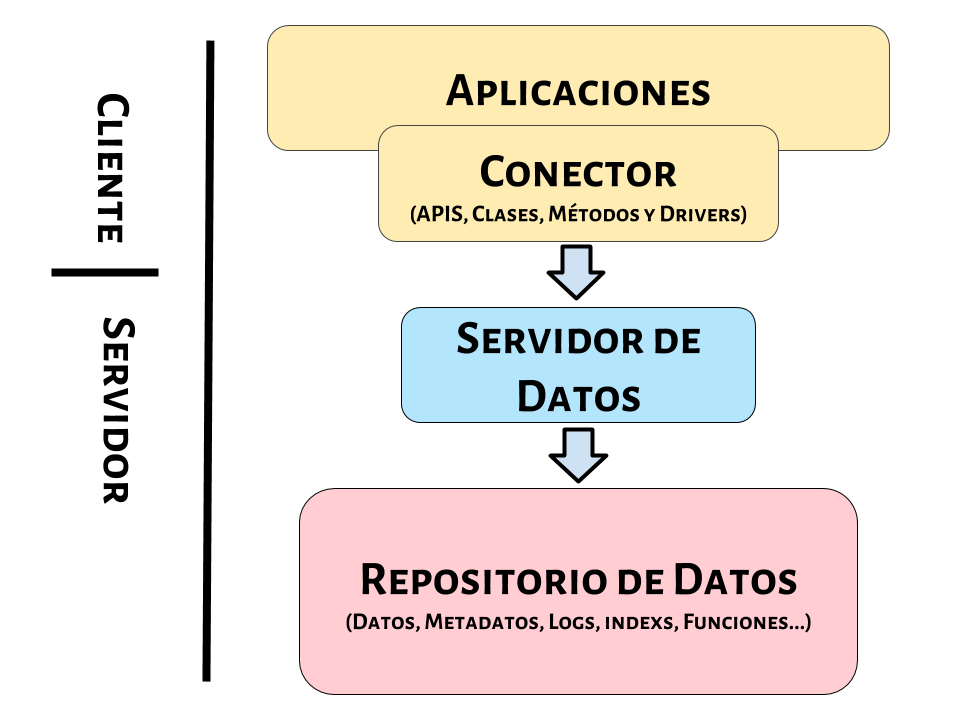
\includegraphics[width=0.85\textwidth]{DiagramaPartes.png}

            \begin{itemize}
                \item
                    \textbf{Aplicaciones:} Es la interfaz entre la base de datos y el usuario, estas pueden
                    ser desarrolladas por un lenguaje de alto nivel 

                \item
                    \textbf{Conector:} Son los componentes que permiten el enlace entre el SGBD y las
                    interfaces desarrolladas en un lenguaje de programación, estas contienen las clases
                    y/o funciones necesarias para llevar a cabo la comunicación entre las aplicaciones
                    con el Sistema Gestor de Base de Datos.

                \item
                    \textbf{Sistema Gestor de Base de Datos:} Son el software especialízado que
                    nos permite manipular inteligentemente nuestro datos:

                    Es la aplicación que permite a los usuarios definir, crear y mantener la base
                    de datos y proporciona acceso controlado a la misma.

                    \begin{itemize}
                        \item Creación de Repositorios
                        \item Creación de Cuentas de Usuarios
                        \item Se encarga de crear archivos lógicos, físicos y objetos de la BD.
                        \item Se encarga de administrar las transacciones, bloqueos , etc.
                    \end{itemize}

            \end{itemize}




        % ==============================================
        % ========   ABSTRACCIÓN DE LOS DATOS   ========
        % ==============================================
        \clearpage
        \section{Abstracción de los Datos}

            \begin{itemize}
                \item
                    \textbf{Nivel Físico}: 

                    Es el nivel base de abstracción que describe como es que la información
                    es guardade de manera actual. Esto nos permite describir como de complejo
                    es que son las estructuras en la realidad.

                \item
                    \textbf{Nivel Lógico}: 

                    Es el nivel que nos muestra como es que se almacena la información dentro de
                    la base de datos y como es que se da la relaciones entre la información.

                    Aunque la implementación de las estructuras simples en el nivel lógico puede
                    implicar complejas estructuras de nivel físico, el usuario de este nivel no
                    necesita ser consciente de esta complejidad.
                    Esto se conoce como independencia de datos físicos. 
                    Los administradores de bases de datos, que deben decidir qué información debe
                    conservar en la base de datos, utilizan el nivel lógico de abstracción.

                \item
                    \textbf{Nivel Visual}: 

                    El nivel más alto de abstracción describe sólo una parte de la base de datos completa.

                    Aunque el nivel lógico utiliza estructuras más simples, la complejidad se mantiene
                    debido a la variedad de información almacenada en una base de datos grande.

                    Muchos usuarios del sistema de base de datos no necesitan toda esta información, 
                    sólo necesitan acceder a una parte de la base de datos.
                    El nivel de vista de la abstracción existe para simplificar su interacción
                    con el sistema.

            \end{itemize}



        % ===============================================
        % ====     USUARIOS DE UNA BASE DE DATOS     ====
        % ===============================================
        \clearpage
        \section{Usuarios de una Base de Datos}


            Hay cuatro grupos de personas que intervienen en el entorno de un sistema de base de datos:
            el administrador de la base de datos, los diseñadores de la base de datos, los programadores
            de aplicaciones y los usuarios.

            \begin{itemize}

                \item
                    \textbf{Diseñadores de la Base de Datos}

                    \begin{itemize}
                        \item Encargado de grabar los propios Módelos de Datos
                        \item Esquema de la Base de Datos
                        \item Diseño lógico de la Base de Datos
                    \end{itemize}


                \item
                    \textbf{Administrador de la Base de Datos}

                    Encargado de: 

                        \begin{itemize}
                            \item Monitorear el Performance
                            \item Diseño físico de la base de datos y de su implementación.
                            \item Herramientas Administrativas
                                \begin{itemize}
                                    \item Creacion de cuentas de usuarios
                                    \item Objetos accedidos.
                                    \item Matriz de autorizacion.
                                \end{itemize}
                            \item Definir tiempos de respaldo
                            \item Reorganización físico
                            \item Llevar a cabo las tecnicas de recuperación
                        \end{itemize}

                \item
                    \textbf{Programadores de Aplicaciones}

                    Son los que se encargan de implementar los programas de aplicación que
                    servirán a los usuarios finales. Estos programas son los que permiten
                    consultar datos, insertarlos, actualizarlos y eliminarlos.

                    \begin{itemize}
                        \item Interfaces de los usuarios finales
                        \begin{itemize}
                            \item Facilitar el acceso a ciertos "objetos" de la BD
                        \end{itemize}

                        \item Interfaces para la gestión de la aplicaciones 
                        \begin{itemize}
                            \item Operaciones de escritura sobre altas ó bajas 
                            \item IDE desarrollo (Java, .NET)
                            \item Lenguaje Scripts
                            \item Conectividad servidores de datos (API s) 
                        \end{itemize}
        
                    \end{itemize}


            \end{itemize}


            % ==================================
            % ====     USUARIOS FINALES     ====
            % ==================================
            \clearpage
            \subsection{Usuarios Finales}

                Los usuarios finales son los clientes de la base de datos, son las personas que
                requieren acceso a la base de datos para realizar consultas, actualizaciones e
                informes. Los usuarios se pueden clasificar en varias categorías:
                \begin{itemize}
                        \item
                            \textbf{Casuales}
                            Estos acceden ocasionalmente a la base de datos, pero pueden necesitar una
                            información diferente en cada momento.

                            \begin{itemize}
                                \item Data Minning
                                \item Big Data
                            \end{itemize}

                        \item 
                            \textbf{Principiantes - Paramétricos}
                            Constituyen una parte considerable de los usuarios finales de los
                            sistemas de bases de datos. Su labor principal gira entorno a la
                            consulta y actualización constantes de la BD.

                        \item 
                            \textbf{Sofisticados}
                            \begin{itemize}
                                \item Experiencia en aplicaciones 
                                \item Programadores de aplicación
                                \item DBA 
                                \item Investigadores
                             \end{itemize}
                            
                        \item 
                            \textbf{Independientes (Stand Alone)} 
                                \begin{itemize}
                                    \item Sistemas Escolares
                                    \item Sistemas de prueba
                                    \item Sin conectividad a otros nodos
                                \end{itemize}

                \end{itemize}






        % ===============================================
        % ===========     DML VS DDL      ===============
        % ===============================================
        \clearpage
        \section{DML vs DDL}

            \begin{itemize}

                \item
                    \textbf{DML}

                        Data Manipulation Languaje, es un lenguaje que nos permite modificar los
                        datos guardados.

                        Los tipos de acceso que tenemos disponibles son:

                        \begin{itemize}
                            \item Recuperar información
                            \item Insertar nueva información
                            \item Eliminar la información
                            \item Modificación de la información
                        \end{itemize}

                    Una consulta o query es una sentencia que solicita la recuperación de información.
                    La parte de un DML que implica recuperación de información se denomina lenguaje
                    de consulta.

                    Aunque técnicamente incorrecto, solemos utilizar los términos lenguaje de consulta
                    y lenguaje de manipulación de datos como sinónimos.


                \item
                    \textbf{DDL}

                    Data Definition Languaje, es Lenguaje de definición de datos.

                    Especificamos un esquema de base de datos mediante un conjunto de definiciones
                    expresadas por un lenguaje especial denominado DDL.

                    El DDL también se utiliza para especificar propiedades adicionales de los datos.

            \end{itemize}
            \clearpage


            Podemos simplificar en el sentido de SQL que:

            \textbf{DDL: Data Definition Language}, mediante el cual puede definir nuevos objetos
            de base de datos, como Table, Views, Stored Procedures, etc.
            Algunos comandos comunes son:

            \begin{itemize}
                \item CREATE
                \item ALTER
                \item DROP
                \item etc...
            \end{itemize}


            \textbf{DML: Data Manipulation Language}, mediante el cual puede realizar cambios en
            los objetos creados anteriormente por DDLs. Algunos comandos comunes son:

            \begin{itemize}
                \item INSERT
                \item UPDATE
                \item DELETE
                \item SELECT
                \item etc...
            \end{itemize}




        % ===============================================
        % ====     ARQUITECTURA DE SISTEMA DE DB    =====
        % ===============================================
        \clearpage
        \section{Arquitectura del Sistema Gestor}

            Podemos acceder al Sistema Gestor de nuestra Base de Datos de muchas maneras, 
            desde formularios web, aplicaciones de escritorio e interpretes de SQL, todos se
            comunican con la Base de Datos mediante SQL.

            \begin{itemize}

                \item
                    \textbf{Motor de Evaluación de Consultas}

                        \begin{itemize}
                            \item Analizador:
                                Este se encarga de analizar las sentencias SQL a nivel
                                sintactico y lexico, así como una validación de que existan
                                dichas relaciones y atributos.

                                Es lo que mucha gente conoce como un compilador de DDL ó DML.

                            \item Evaluador de Operaciones:
                                Este se encarga de crear el árbol canónico, es decir, la forma
                                formal que tendría el árbol necesario para acceder a la información.

                            \item Optimizador:
                                Se encarga de tomar el árbol canónico y optimizarlo para que se tenga
                                que hacer la menor cantidad de operación a nivel lógico, este se conoce
                                como árbol de consulta. 

                            \item Ejecutor de Planes:
                                Se encarga de planear la mejor estrategia para ejecutar la consulta
                                de tal manera que se optimize de manera física.
                        \end{itemize}

                \clearpage
                \item
                    \textbf{Gestores}

                        \begin{itemize}
                            \item Gestor de Transacciones:
                                Este es el que se encarga de organizar varias sentencias SQL para ejecutarlas
                                como una transacción.
                            
                            \item Gestor de Bloqueos:
                                Este es el que se encarga de ver si es que cierta relación 
                                esta bloqueada porque esta ocurriendo una transacción en ese momento.

                                Los bloqueos son una parte muy importatne de este gesto.

                                Podemos definirlos en principalmente 2:
                                \begin{itemize}
                                    \item Binario:
                                        Es decir permite que una relación este o bine bloqueada
                                        o no para lectura o escritura.
                                    \item Múltiplos Niveles:
                                        Es decir nos permite que existan bloqueos de lectura,
                                        escritura diferentes, ayudando a evitar las esperas si no
                                        son necesarias.
                                \end{itemize}

                            \item Gestor de Recuperación:
                                Este es el que se encarga de definir todas las técnicas de recuperación
                                sobre la base, estas mismas las podemos definir en dos:
                                \begin{itemize}
                                    \item Inmediatas: Son las que podemos representar como rollback o rollfoward
                                    \item Técnicas en Frío: Usa una copia de seguridad
                                \end{itemize}


                            \item Gestor de Archivos y Métodos de Acceso
                                Todos los elementos, metadatos, logs, funciones, etc... tienen que estar
                                almacenada de manera física.

                                Este se encarga de dependiendo de las querys como es que debe acceder de 
                                manera eficiente a los datos.

                            \item Gestor de Memoria Intermedia
                                Es como una RAM, nos permite guardar consultas bastante frecuentes
                                para aumentar la velocidad sobre la RAM
                        \end{itemize}

            \end{itemize}


            \begin{figure}[h!]
                \centering
                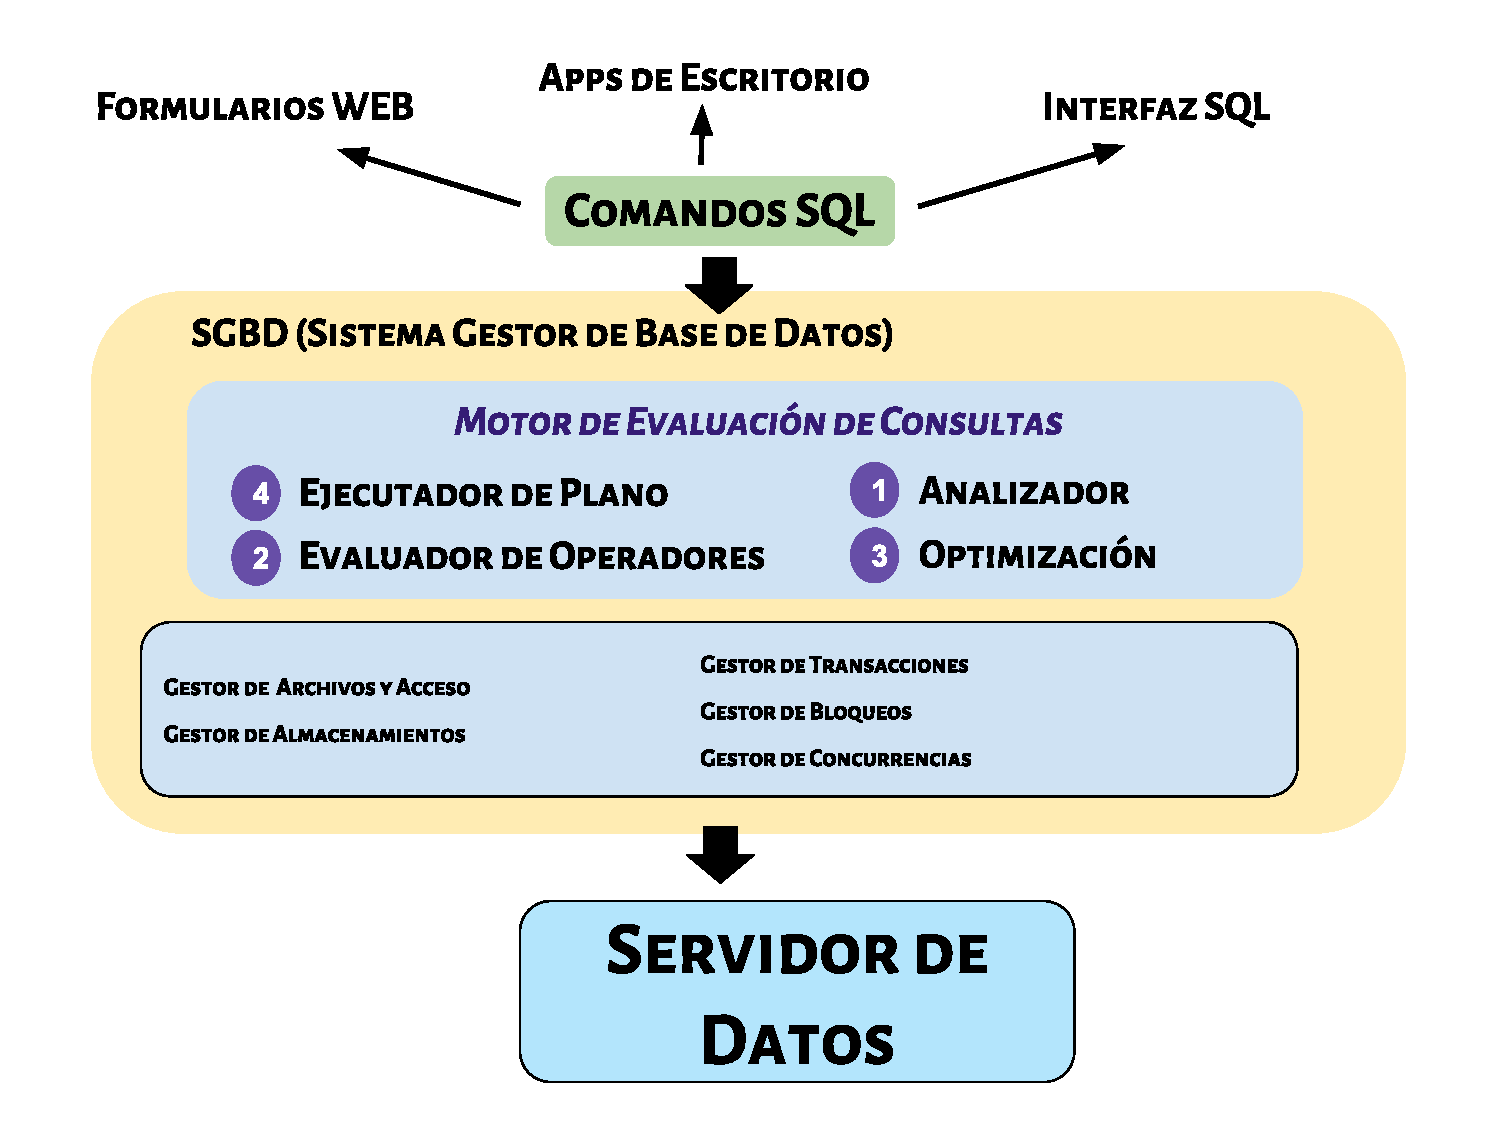
\includegraphics[width=0.65\textwidth]{ArquitecturaSGBD.pdf}
            \end{figure}







        % ===============================================
        % ====     ARQUITECTURA DE BASES DE DATOS   =====
        % ===============================================
        \clearpage
        \section{Arquitecturas de las Bases de Datos}


            \begin{itemize}

                \item
                    \textbf{Cliente - Servidor}

                    Mientras que el servidor es aquel que contiene toda la información 
                    importante, el cliente solo se encarga de solicitar servicios.

                    Podemos seperar estos como:
                    \begin{itemize}
                        \item Cliente sin Disco:
                            Aquel que puede acceder a la información pero no puede modificarlo.

                        \item Cliente con Disco:
                            Aquel que puede acceder a la información y puede modificarlo.
                     \end{itemize} 


                \item
                    \textbf{Multibase}

                    Esta se caracterisa porque cada base de datos interna que tienes no se relaciona
                    entre si, es decir, no hay comunación entre ellas.

                        
            \end{itemize}





    % ===============================================================================
    % ===================        SISTEMA RELACIONAL         =========================
    % ===============================================================================
    \chapter{Modelos de Datos}


        % =========================================================
        % =========     MODELO ENTIDAD RELACION      ==============
        % =========================================================
        \clearpage
        \section{Sistema Entidad-Relación}

            Fue creado por Peter Pin‐Shan Chen en 1976, llamado \Quote{The Entity Relationship
            Model Toward Unified View of Data}

            Es un modelo conceptual, es decir, creado en lenguaje natural y se se ayuda 
            de DER (gráficas) para hablar de las relaciones.

            Permite construir el modelo conceptual de datos.
            \begin{itemize}
                
                \item Es una representación de la estructura y contenido de una base de datos.

                \item Es independiente  del software (como el SMBD).
                
                \item Permite establecer las restricciones de la BD.

                \item Esta asociado al modelo de datos que es usado para implementar la BD.

            \end{itemize}

            Siendo una publicado por la ACM (Association for Computing Machinery), 
            considera los siguientes puntos:

            \begin{itemize}
                \item Incorpora información semántica del mundo real.

                \item Introduce una técnica gráfica como herramienta para el diseño
                    de bases de datos (Diagrama Entidad Relación).

                \item Es una representación lógica de los datos de una organización o
                    un área de negocio.

                \item Normalmente es expresado como un DER, siendo este la representación
                    gráfica del Modelo ER.
            \end{itemize}


            % ==============================================
            % =========      ENTIDADES             =========
            % ==============================================
            \clearpage
            \subsection{Entidades}
                    
                Son objetos que existen en el mundo real y que son distingubles
                (gracias a sus características) de otros objetos.

                El tipo de entidad es el esquema que tiene la entidad en la base de datos,
                es decir son todos los atributos o características que definien a la entidad.

                Piensa en las entidades como sustantivos.
                Ejemplos: cliente, estudiante, automóvil o producto. 


                \begin{figure}[h]
                    \centering
                    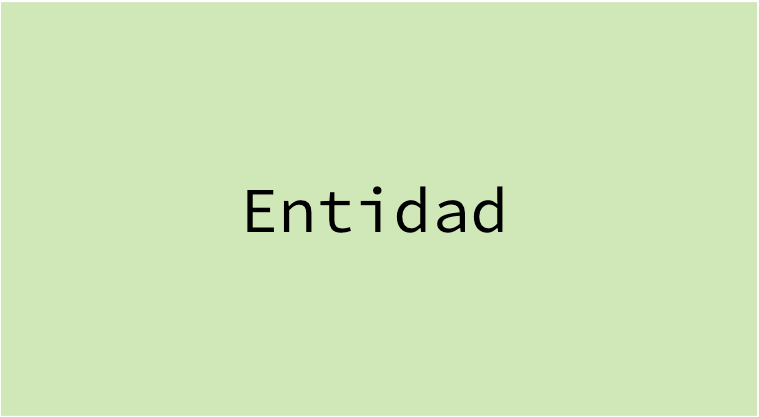
\includegraphics[width=0.30\textwidth]{Entidad0}
                    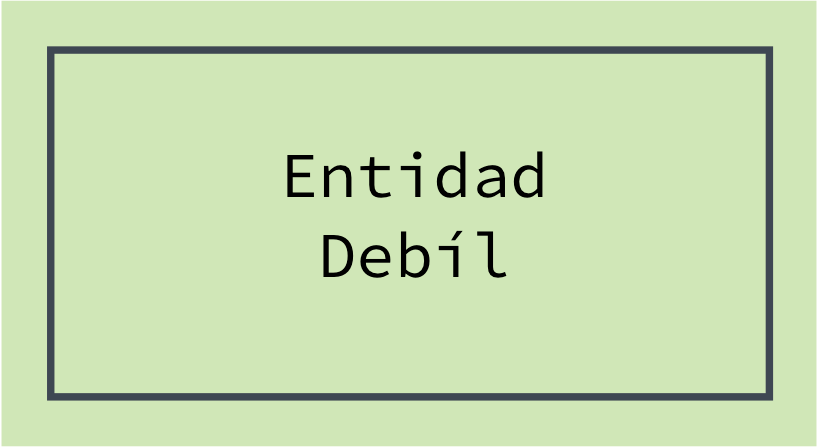
\includegraphics[width=0.30\textwidth]{Entidad1}
                    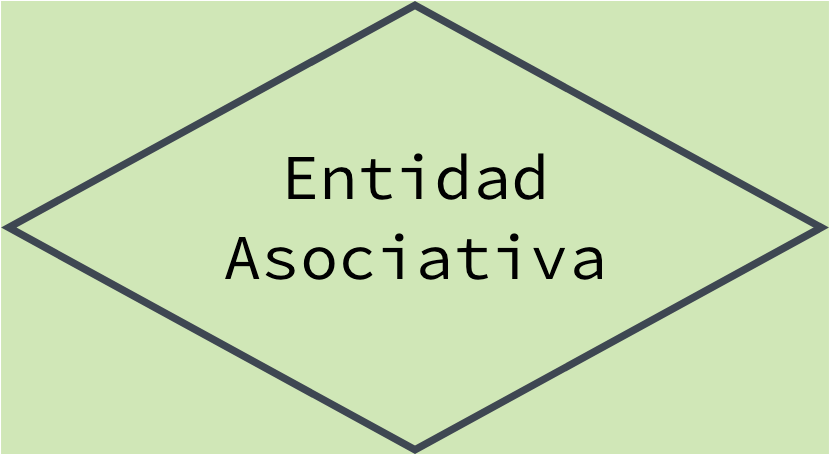
\includegraphics[width=0.30\textwidth]{Entidad2}
                \end{figure}


                \begin{itemize}
                    \item Fuerte:\\
                        Es aquella entidad cuya existencia no depende de otras entidades.
                    \item 
                        Debíl:\\
                        Es aquella entidad cuya existencia depende de otras entidades.
                        \begin{itemize}
                            \item Esta depende de de una o varias entidades fuertes
                            \item Una entidad debíl jamas se debe asociar con una entidad debíl
                            \item Una entidad debíl no tiene identificador propio, pero si parciales
                            \item Usa una relación identificada para asociar una entidad fuerte con una debíl
                        \end{itemize}


                    \item Asociativa: \\
                        Se usa cuando tienes una relación y resulta que quieres usar esta relación
                        como conexión (por ejemplo la relación entre alumno y clase) así que haces
                        esa relación una entidad asociativa (por ejemplo para asociar esta nueva
                        entidad con profesor).
                \end{itemize}



            % ==============================================
            % =========      RELACIONES            =========
            % ==============================================
            \clearpage
            \subsection{Relaciones}
                    
                Esto es como las entidades actúan unas sobre otras o están asociadas entre sí.
                Piensa en las relaciones como verbos.

                Por ejemplo, el estudiante nombrado puede registrarse para un curso.
                Las dos entidades serían el estudiante y el curso, y la relación representada es
                el acto de inscribirse, conectando las dos entidades de esa manera. 

                \begin{figure}[h]
                    \centering
                    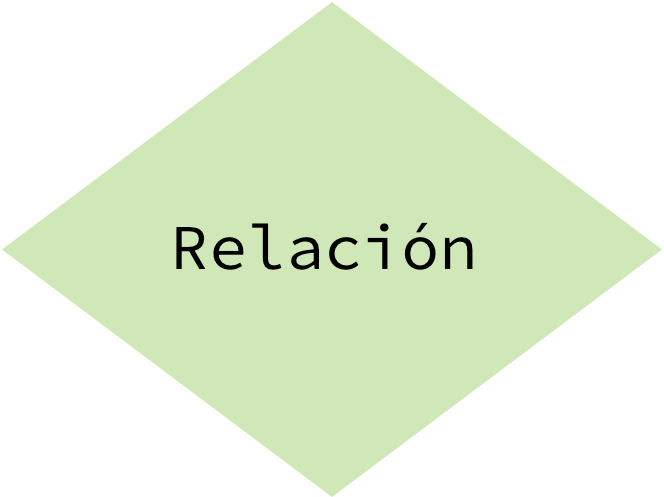
\includegraphics[width=0.40\textwidth]{Relacion0}
                    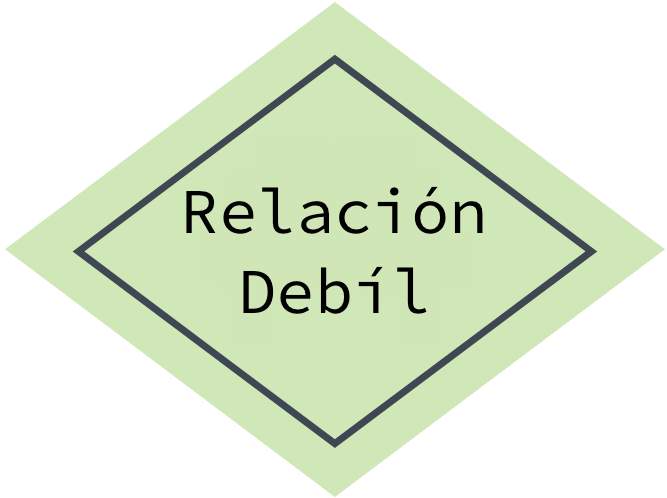
\includegraphics[width=0.40\textwidth]{Relacion1}
                \end{figure}


            % ==============================================
            % =========      CARDINALIDAD          =========
            % ==============================================
            \subsection{Cardinalidad}

                Nos dice la cantidad de atributos que se relacionan.


                \begin{figure}[h]
                    \centering
                    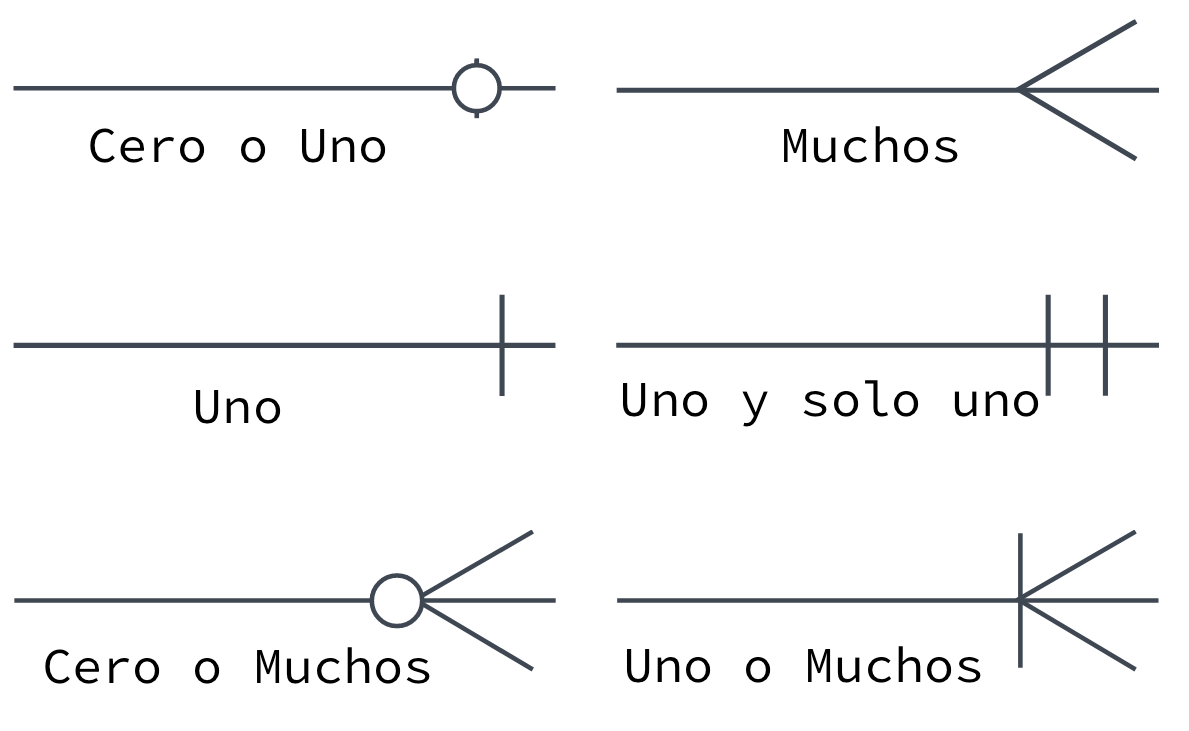
\includegraphics[width=0.80\textwidth]{Cardinalidad}
                \end{figure}


            % ==============================================
            % =========      ATRIBUTOS             =========
            % ==============================================
            \clearpage
            \subsection{Atributos}

                Son las propiedades o características de una entidad
                \begin{itemize}
                    \item Identificador:
                        Es aquel atributo que nos permite identificar de forma unica cada una de las
                        instancias de la entidad.

                        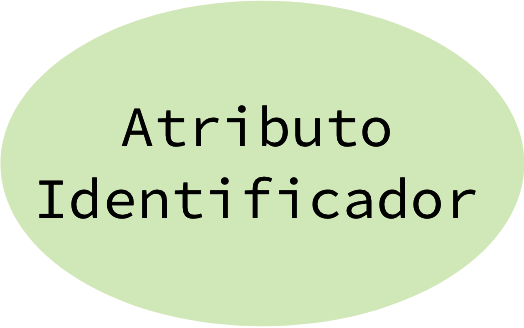
\includegraphics[width=0.20\textwidth]{Atributos1}

                    \item Simples:
                        Son aquelllas propiedades atomicas que ya no se pueden subdividir
                        
                        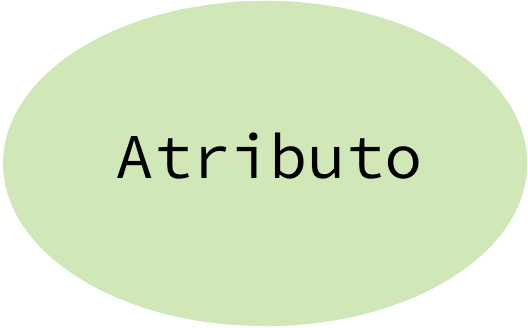
\includegraphics[width=0.20\textwidth]{Atributos0}


                    \item Derivado:
                        Es aquel que se puede calcular con la información que ya tenemos
                        como la edad con la fecha de nacimiento

                        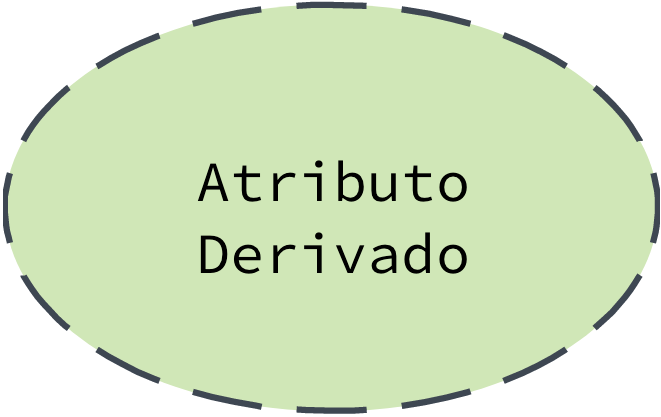
\includegraphics[width=0.20\textwidth]{Atributos3}

                    \item Multivalor:
                        Aquellos que tienen mas de un valor

                        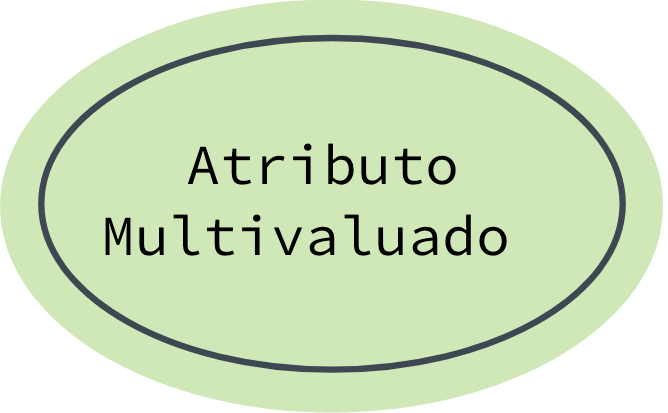
\includegraphics[width=0.20\textwidth]{Atributos4}


                    \item Compuestos :
                        Aquellos que estan formados por varios sub atributos

                \end{itemize}







        % ========================================================
        % ========    MODELO EXTENDIDO ENTIDAD RELACION    =======
        % ========================================================
        \clearpage
        \section{Sistema Entidad-Relación Extendido}

            \begin{wrapfigure}{r}{0.18\textwidth}
                \centering
                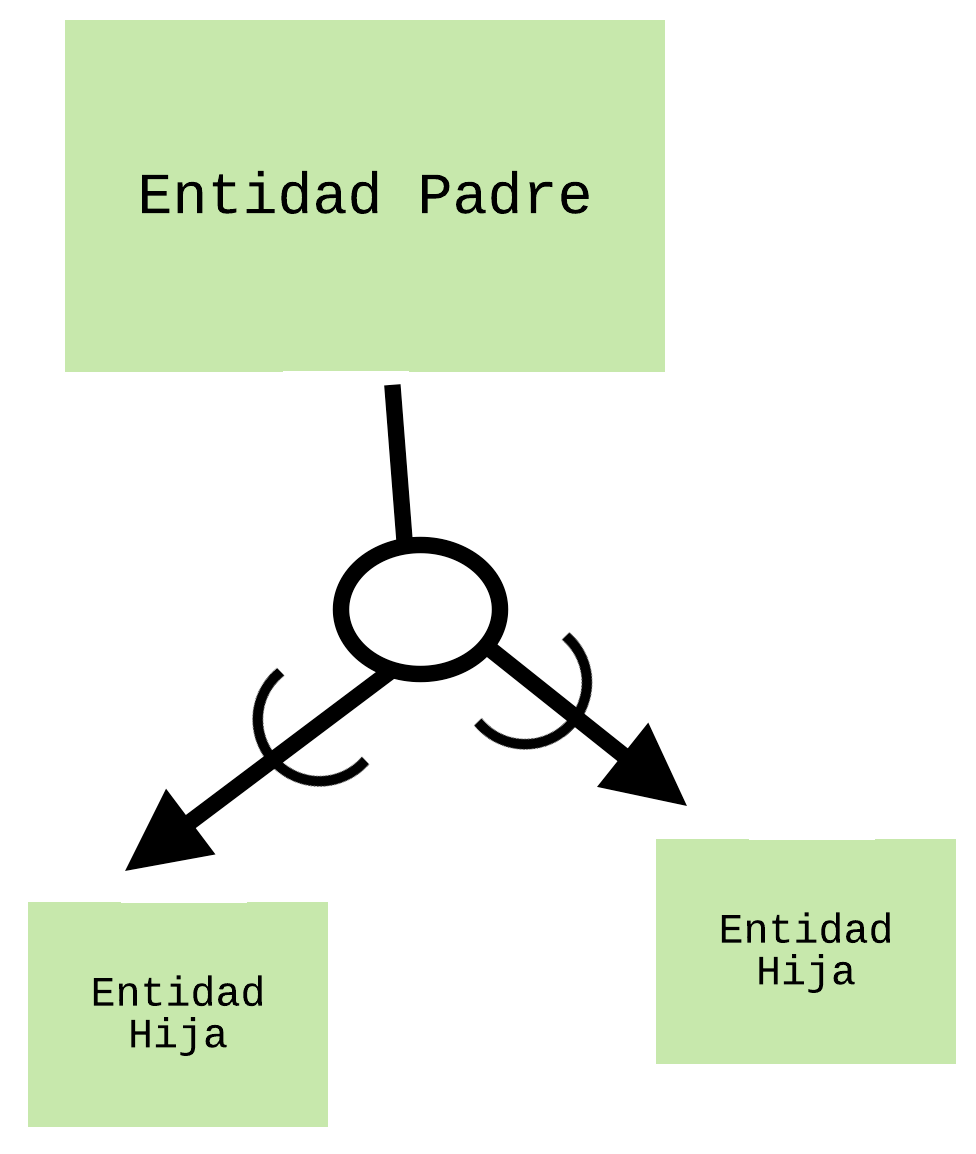
\includegraphics[width=0.16\textwidth]{EERD0}
            \end{wrapfigure}

            El Modelo de Relación de Entidad Extendida es un modelo más complejo y de más
            alto nivel que extiende un diagrama E-R para incluir más tipos de abstracción
            y para expresar más claramente las restricciones.

            Todos los conceptos de un diagrama E-R están incluidos en el modelo EE-R.

            Vamos a ver las diferencias más importantes con respecto a nuestro clásico amigo
            el diagrama entidad relación.

            \begin{itemize}
                \item
                    \textbf{Herencia: Super y Subclases}

                    Como el nombre sugiere, podemos tener entidades que consideramos padres
                    y que heredan a otras entidades hijas.

                    Por ejemplo podemos podemos tener una entidad empleado puede tener
                    subentidades que se dividen por el trabajo que hacen, por ejemplo
                    diseñadores, gerentes y ayudantes.

                    Todas nuestras subentidades van a heredar las propiedades o atributos
                    de nuestra superentidad.

                    Esto nos permite que nuestra entidad padre sea una idea general y que
                    nuestras subclases sean especializaciones de la misma, por esto decimos
                    que esta clase de diagramas permite la especialización.


                    Es también importante remarcar que alguna de nuestras entidades
                    puede heredar de una o mas entidades


                \item
                    \textbf{Generalización y Especialización}

                    Como habiamos hablando antes, esto nos permite que si tenemos
                    una gran cantidad de entidades con atributos comunes podemos 
                    crear una entidad general y hacer que las demás hereden de ella,
                    con esto también propiciamos que nuestras entidades que heredan 
                    se puedan especializaciar.


                \item
                    \textbf{Restricciones}
                        Tambien es común que se les conozca como superclass constraint

                        \begin{itemize}
                            \item Entidades Disconjuntas
                            \item Entidades Superpuestas
                        \end{itemize}

                \clearpage


                \item
                    \textbf{Discriminadores de Superentidad}

                    Un discriminador de entidades es un atributo que indica el subtipo
                    de una entidad.

                    Es decir podemos indicar con este diagrama si las divisiones que hacemos
                    son parciales (es decir, es posible que una instancia de la sueprclase
                    pueda existir sin tener que ser parte de una subentidad) o total
                    en la que decimos que cualquier instancia tiene que pertencer a alguna
                    subentidad

                    \begin{figure}[h]
                        \centering
                        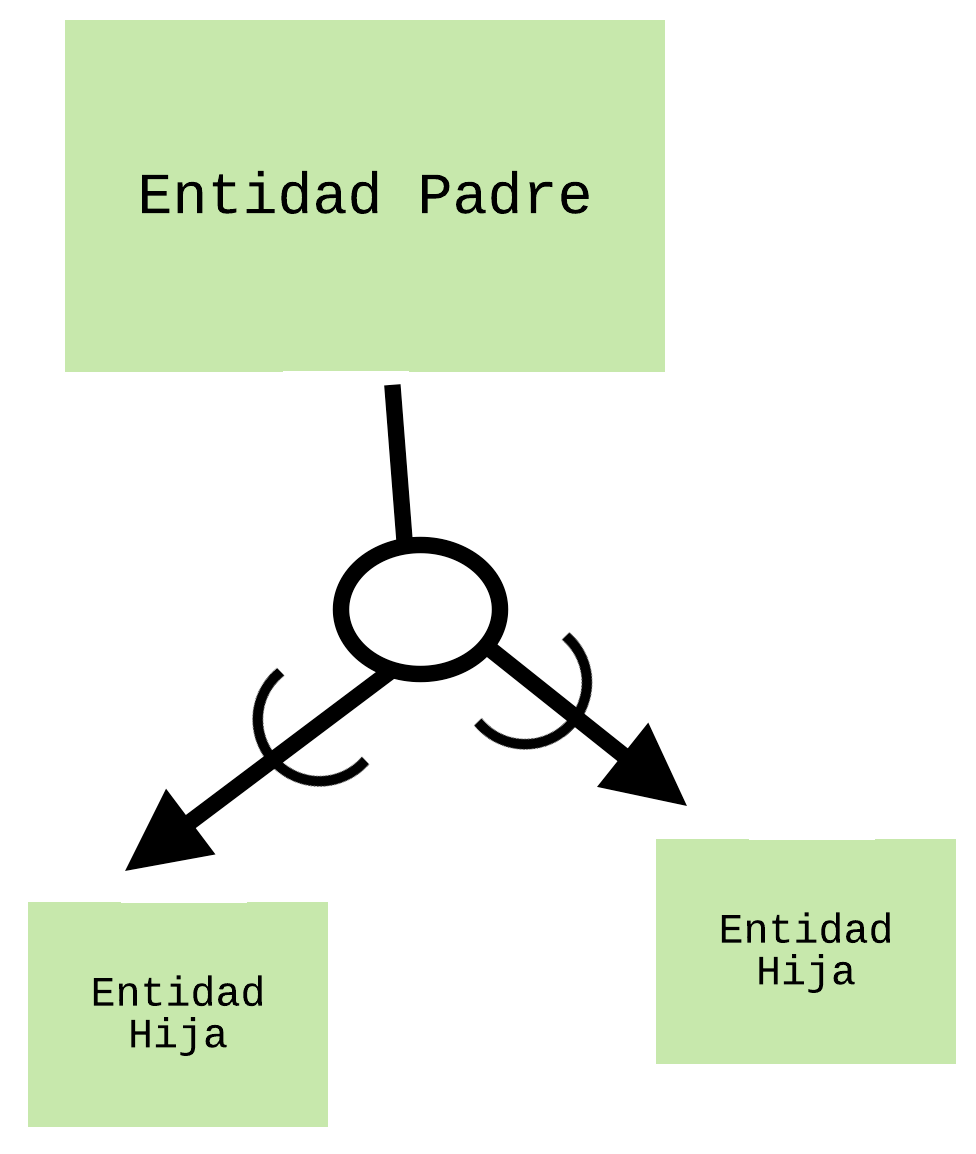
\includegraphics[width=0.30\textwidth]{EERD0}
                        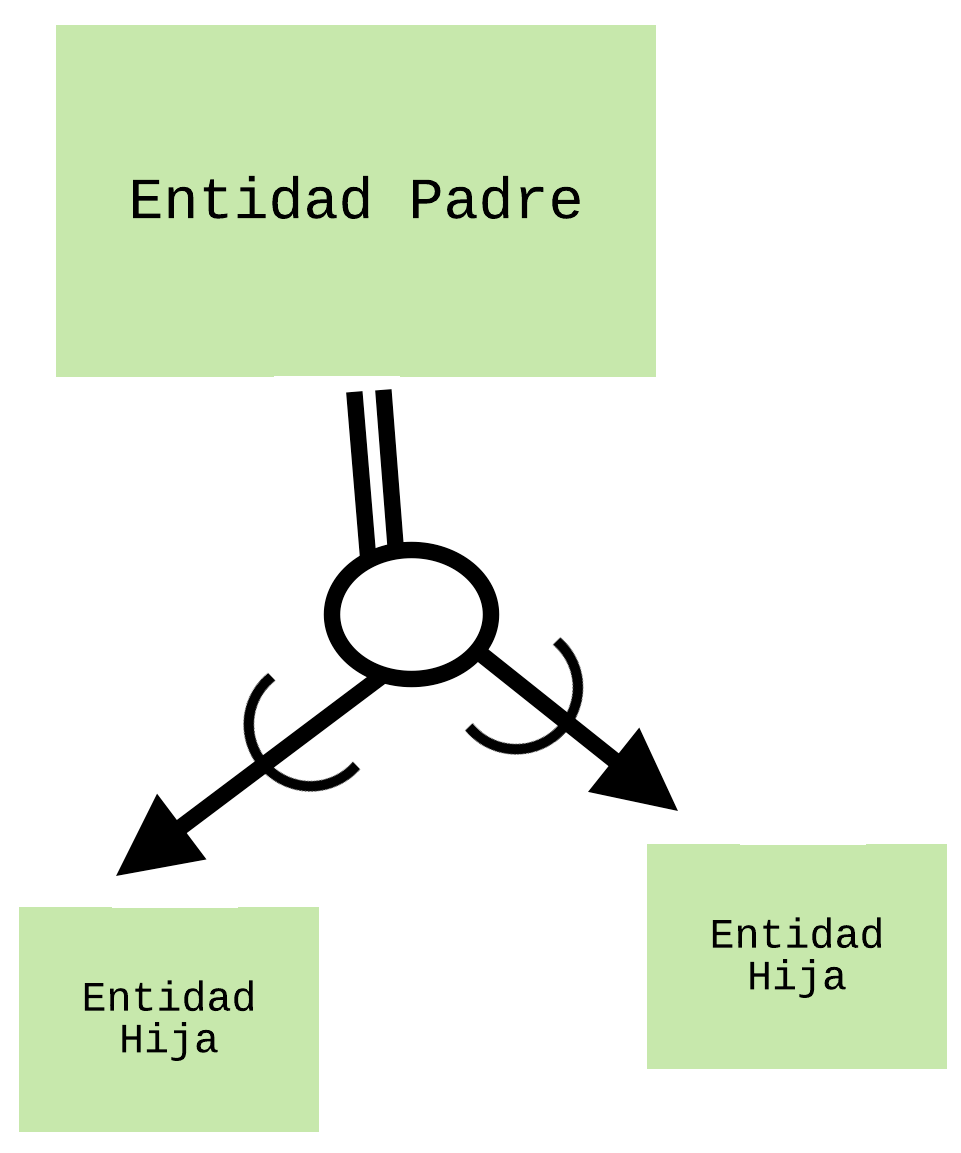
\includegraphics[width=0.30\textwidth]{EERD1}
                    \end{figure}

            \end{itemize}







        % ========================================================
        % ============    SISTEMA RELACIONAL     =================
        % ========================================================
        \clearpage
        \section{Sistema Relacional}

            Las bases de datos relacionales facilitan evitar la duplicidad de información
            e inconsistencias de datos.
            La mayoría de los sistemas de bases de datos utilizados hoy en día son relacionales.

            En el modelo relacional, los datos se dividen en diferentes \textbf{tables}.
            Una tabla funciona como una matriz o una hoja de cálculo.

            Normalmente, las columnas imponen un tipo de datos que pueden contener.
            Las columnas también pueden especificar otras restricciones: si es obligatorio que las
            filas tengan un valor en esa columna, si el valor de la columna debe ser único en todas
            las filas y cosas así.

            Las columnas se denominan más comúnmente atributos.
            Si una columna sólo permite números enteros, decimos que es un campo entero.
            Diferentes tablas utilizan diferentes tipos de campos.

            La organización de una tabla de base de datos viene dada por sus campos y las
            restricciones que imponen.

            Todas las entradas de datos son filas y el sistema de base de datos no aceptará
            una fila en una tabla si viola el esquema de la tabla. Esa es una gran limitación
            del modelo relacional.
            Cuando las características de los datos varían demasiado, la adaptación de los datos
            a un esquema fijo puede ser problemática. Pero si está trabajando con datos de
            estructura homogénea, un esquema fijo le ayudará a garantizar que los datos son válidos.



            % ==============================================
            % =========      RELACIONES            =========
            % ==============================================
            \clearpage
            \subsection{Relaciones}

                Para evitar la redundancia de datos la clave esta en crear diversas tablas
                e ir relacionandolas.

                Para lograr esto tenemos que crear relaciones, y es imposible hablar de relaciones
                sin hablar de llaves:


                \begin{itemize}
                    \item
                        \textbf{Primary Key:}
                        La idea de una llave primaria es crear un atributo que tiene, tiene pero
                        tiene que ser único y es recomendable que casi no cambie.


                    \item
                        \textbf{Foreign Key:}
                        La idea de una llave secundaria es crear un atributo que tiene que alguna otra
                        tabla sea la llave primaria. Eso es todo.

                \end{itemize}


 










            
        





    % ===============================================================================
    % =========================           S Q L                ======================
    % ===============================================================================
    \chapter{SQL}

        % ==============================================
        % ========      SQL COMO LENGUAJE      =========
        % ==============================================
        \clearpage
        \section{SQL como Lenguaje}
            
            SQL \textbf{no} es tan potente como una máquina universal de Turing.

            Es decir, hay algunos cálculos que son posibles utilizando un lenguaje de programación
            de propósito general, pero no son posibles con SQL.
            SQL también no admite acciones como la entrada de usuarios, la salida a las pantallas 
            ó la comunicación a través de la red.
            Dichas computaciones y acciones deben escribirse en un lenguaje principal (C, C++ ó Java)
            con consultas SQL incorporadas que acceden a los datos de la base de datos

            Los programas de aplicación son programas que se utilizan para interactuar con la base de datos de esta manera.








% //////////////////////////////////////////////////////////////////////////////////////////////////////////
% ///////////////////////////////////         PARTE PRACTICA               /////////////////////////////////
% //////////////////////////////////////////////////////////////////////////////////////////////////////////
\part{Parte Practica}
\clearpage


    % ===============================================================================
    % ===================        QUERIES EN SQL                ======================
    % ===============================================================================
    \chapter{Queries en SQL}
    \clearpage

        % ========================================
        % =========   SELECT FROM    =============
        % ========================================
        \section{SELECT FROM}

            Empecemos por la sentencia más básica para un Query en SQL:

            \begin{lstlisting}[language=SQL, gobble=16]
                SELECT FielName FROM TableName;
            \end{lstlisting}

            Ahora empecemos por aquí:
            \subsection{Distint vs All}
            \begin{itemize}
                \item Distint (Default):
                    Esta solo muestra solo los atributos diferentes

                    \begin{lstlisting}[language=SQL, gobble=24]
                        SELECT DISTINT FielName FROM TableName;
                    \end{lstlisting}
                \item All:
                    Esta muestra todos los atributos, incluso duplicados
                    \begin{lstlisting}[language=SQL, gobble=24]
                        SELECT ALL FielName FROM TableName;
                    \end{lstlisting}
            \end{itemize}



        % ========================================
        % =========   COUNT , AVE, SUM  ==========
        % ========================================
        \section{Funciones de Agregación}

            Las funciones de agregación son funciones que toman una colección
            como entrada y regresan un simple valor. SQL ofrece estas 5 funciones
            por default:

            \begin{itemize}
                \item \Quote{AVG()}: Promedio
                \item \Quote{MIN()}: Minimo
                \item \Quote{MAX()}: Máximo
                \item \Quote{COUNT()}: Cuenta la cantidad 
                \item \Quote{SUM()}: Suma todo el resultado
            \end{itemize}





        % ========================================
        % ============     WHERE   ===============
        % ========================================
        \clearpage
        \section{WHERE}

            Esta nos permite seleccionar solo las filas en el resultado del quey
            que satisface nuestros criterios.

            \begin{lstlisting}[language=SQL, gobble=16]
                SELECT FielName FROM TableName
                    WHERE
                        (TableName.Thing1 < Something) AND
                        (TableName.Thing2 = "Some Strings");
            \end{lstlisting}

            Tenemos a nuestra dispoción los siguientes comparadores:
            \begin{itemize}
                \item Lógicos: AND, OR, NOT
                \item Aritmeticos: <, >, <=, >=, =, <>
            \end{itemize}



        % ========================================
        % ============   STRINGS   ===============
        % ========================================
        \section{Comparación de Strings}
            
            Podemos comparar strings gracias a lo que conocemos como comodínes usando
            el comando \Quote{LIKE}
            \begin{itemize}
                \item \Quote{\%}: Que sirve como comodín para cualquier cantidad de caracteres 
                \item \Quote{\_}: Que sirve como comodín para un caracter 
            \end{itemize}


        % ========================================
        % ========   ORDEN DE TUPLAS   ===========
        % ========================================
        \section{Orden de las Tuplas}

            Podemos controlar el orden en que se nos retornan las tuplas del query que estamos
            haciendo muy facilmente con la instructiva ORDER BY.

            Por default se usa la opción \Quote{ASC} que las ordena de manera ascendente
            mientras que \Quote{DESC} la ordena de manera descendente.

            Por default esta se coloca la última línea de manera implicita:
            \begin{lstlisting}[language=SQL, gobble=16]
                SELECT DISTINT FielName1, FielName2, FielName3 FROM TableName
                    ORDER BY FielName1 ASC, FielName2 ASC, FielName3 ASC;
            \end{lstlisting}

            También podemos simplemente poner el número en que las pusimos para 
            indicar el orden:

            \begin{lstlisting}[language=SQL, gobble=16]
                SELECT DISTINT FielName1, FielName2, FielName3 FROM TableName
                    ORDER BY 1,2, 3;
            \end{lstlisting}


    % ===============================================================================
    % ===================        QUERIES EN SQL                ======================
    % ===============================================================================
    \section{Views en SQL}


        En teoría de bases de datos, una vista es una consulta que se presenta como una tabla (virtual)
        a partir de un conjunto de tablas en una base de datos relacional.

        Las vistas tienen la misma estructura que una tabla: filas y columnas.
        La única diferencia es que sólo \textbf{se almacena de ellas la definición, no los datos}.
        Los cambios aplicados a los datos en una tabla se reflejan en los datos mostrados en invocaciones
        posteriores de la vista.
        En algunas bases de datos NoSQL, las vistas son la única forma de consultar datos.

        Los datos que se recuperan mediante una consulta a una vista se presentarán igual que los de una tabla.

        Una vista se crea a través de una expresión de consulta (una sentencia SELECT) que la calcula y que puede
        realizarse sobre una o más tablas.


        % ========================================
        % =========     VENTAJAS     =============
        % ========================================
        \subsection{Ventajas}

            Las vistas pueden ofrecer ventajas sobre las tablas:

            \begin{itemize}

                \item
                    Las vistas pueden representar un subconjunto de los datos contenidos en una tabla.
                    En consecuencia, una vista puede limitar el grado de exposición a las tablas al mundo exterior:
                    un usuario dado puede tener permiso para consultar la vista, mientras que se deniega el acceso
                    al resto de la tabla base.

                \item
                    Las vistas pueden ocultar la complejidad de los datos.
                    Por ejemplo, una vista podría aparecer como Sales2000 o Sales2001, particionando
                    de forma transparente la tabla subyacente real.

                \item 
                    Las vistas cuestan muy poco espacio para almacenar; la base de datos contiene sólo
                    la definición de una vista, no una copia de todos los datos que presenta.

            \end{itemize}



        % ========================================
        % =========    SINTAXIS      =============
        % ========================================
        \subsection{Sintaxis}

            Empecemos por la sentencia general de las vistas:

            \begin{lstlisting}[language=SQL, gobble=16]
                CREATE VIEW ViewName AS
                    SELECT FielName
                        FROM TableName
                        WHERE Conditions
                        ORDER BY FielName; 
            \end{lstlisting}

\end{document}




























